%===============================================
\programme{Coal, Biomass, Heavy Oil}
%===============================================

%=====================================
\section*{Function}
%=====================================

Pulverised coal combustion is described (excluding grid burning) allowing the
use of mixture of coals (or of coal and biomass) and a description of
granulometry (as many classes of initial diameter as wished). After a particle
enters the furnace, radiation increases its temperature.
\begin{enumerate}
\item As particle's temperature increases, evaporation of free water (if any)
  begins. During evaporation, the vapor pressure gradient extract some water
  from the particle. The interfacial mass flux brings some mass, water and
  enthalpy (computed for water vapour) then latent heat is taken from the
  particle's enthalpy so the heating is slowed (during evaporation, the water
  can't reach the boiling point). Fuel oil is supposed to be dry.
\item After drying is achevied, the temperature reaches higher level, allowing
  the pyrolysis phase to take place. The pyrolysis is described by two
  competitive reactions : the first one with a moderate activation energy is
  able to free peripherals atoms group from skeleton leaving to light gases and
  a big amount of char ; the second one with an higher activation enrgy is able
  to break links deeper in the skeleton leaving to heavier gases (or tar) and
  less char (more porous). So a complete description needs two sets of three
  parameters (two kinetics ones and a partitioning one):
\begin{eqnarray}
\mbox{Coal} &=&(k_{01}~,~ T_{01}) ~\Rightarrow~ Y1~\{ \mbox{Light Volatiles~~}\} ~+~ (1-Y1)~\{ \mbox{Char} \} \\
\mbox{Coal} &=&(k_{02}~,~ T_{02}) ~\Rightarrow~ Y2~\{\mbox{Heavy Volatiles~} \}   ~+~ (1-Y2)~\{ \mbox{Char} \}
\end{eqnarray}
Where $Y_1$, the partitionning (or selectivity) factor of the "{\em low
  temperature}" reaction is less than $Y_2$, the "{\em high temperature}" one.
A practical rule is to consider that the same hydrogen can bring twice more
carbon by the second reaction than by the first one.When ultimate analysis are
available both for coal and for char, it is relevant to check partioning
coefficient ($Y_{i}$) and composition of volatiles matters (mainly ratio of
Carbon monoxide and C$/$H in the hydrocarbon fraction) : assumptions on
volatiles composition gives partitionning coefficients ; assumptions on $Y_{i}$
determine volatiles equivalent formulae. Pyrolisis interfacial mass flux brings
energy of volatile gases (computed at the particle's temperature) in wihch the
formation of enthalpy of gaseous species differs from the coal one's, as a
result, the enthalpy for pyrolisis reaction (the most ofen, moderate) is taken
from particle energy.\\
The heavy fuel oil undertakes a set of physico-chemical transformation : light
hydrocarbons can evaporate while the heaviest undergo a pyrolisis. With a few
data, only a temperature range is available for mass loss of droplets : the heat
flux is shared out between warming of the remaining liquid and evaporation
enthalpy. At the very end of theses processes a solid particle is leaved, mainly
made of a porous carbon similar to char.
\item After pyrolysis and evaporation, when every volatiles are burnt, oxygen is
  able to reach the surface of the char particle. So heterogenous combustion can
  take place : diffusion of oxygen from bulk, heterogeneous reaction
  (kinetically limited) and back diffusion of carbone monoxide. The
  heterogeneous oxidation interfacial mass flux is the difference of an incoming
  oxygen flux and an outcoming carbon monoxide mass flux, each of them at their
  own temperature. The incoming oxygen has a zero valued formation enthalpy
  (reference state) and the outcoming carbon monoxide has a negative formation
  enthalpy, as a result, the enthalpy liberated by the first oxidation of carbon
  is leaked in the particle energy, contributing to its heating. The
  heterogenous combustion is complete if all the carbon of the char particle is
  converted, leaving an ash particle. Unburnt carbon can leave the boiler as fly
  ash. The heterogeneous reaction is written as following :
\begin{eqnarray}
\mbox{Char} + \displaystyle \frac{1}{2} O_{2} &=& (k_{0,\mbox{\small het}}~,~ T_{0,\mbox{\small het}}) ~\Rightarrow~ CO \qquad
\end{eqnarray}
\item In the same way, after pyrolysis vanishes, gasification can take place by :
\begin{eqnarray}
\mbox{Char} +  CO_{2} &=&(k_{0,\mbox{\small gc}}~~,~ T_{0,\mbox{\small gc}})~~~\Rightarrow~ 2 CO                 \\
\mbox{Char} +  H_{2}O &=&(k_{0,\mbox{\small gw}}~,~ T_{0,\mbox{\small gw}})  ~~\Rightarrow~ CO + H_{2}
\end{eqnarray} 
\end{enumerate}

The 2011 version is able to deal with many class of particles \fort{ncla}, each
class beeing described by an initial diameter and a constituting coal.  Every
coal, among \fort{nchar} is described by a complete set of parameters :
immediate and ultimate analysis, low heating value (at user choice on raw, dry
or pure) and kinetic parameters ({\em for the two competitive pyrolysis reaction
  and for heterogeneous reaction}). This allows to describe the combustion of a
mixture or coals or of coal and every material following the same evolution
kinetics (woods chips ...). It is, obviously, possible to mix fuels with (very)
different proximate analysis, like dry hard coal and wet biomass.\\
Subroutines allowing the user to describe inlets are dedicated to standard
combustion : some inlets are for coal (eventually blend)and a gaseous media,
others for oxidizers. If needed, a deeper modification allows to describe
co-combustion of coal and some gases ... described as volatile matter from a
coal.

The heavy fuel oil injection is described by a thermodynamic data file and
granulometry, neither blend nor coal / oil mixing is possible.

%============================================================================
\section*[Diffusion turbulent reaction]{Enhancement of diffusion turbulent reaction for two phase combustion}
%============================================================================

With a Probability Density Function and the assumption of concentrations
piecewise linear vs. the variable, it is quite easy to integrate and found the
mean concentrations. For gas diffusion flame this is done by \fort{d3pphy,
  d3pint}, it seems more relevant to explain the algorithm in a more complicated
case : for coal, biomass and heavy fuel oil, in \fort{multiphase gas combustion
  five reactions} can be considered.
\begin{enumerate}
\item 1) gases issued from slow phenomena (vs. turbulent mixing) as
  heterogeneous combustion and gasification, both by $CO_{2}$ and $H_{2}O$ are
  mixed with various oxidizers ; if any gasification by $H_{2}O$ has been
  undertaken, some $H_{2}$ is released. This (tiny : an industrial combustor is
  not a gasifier) amount is supposed to recombine as a reaction prior to mixing
  and main turbulent combustion.
\item 2 and 3) Coal is assumed to undergos two competitves pyrolysis reactions,
  the first releasing organic compound summarized as $CH_{x1}$, the second
  releasing $CH_{x2}$ (with $x1 > x2$), both of them releasing $CO$. The first
  reaction to occur in the gas phase is the partial dehydrogenation ( lowering
  saturation) of $CH_{x1}$ to produce water vapor and $CH_{x2}$. Then the
  $CH_{x2}$ (produced by pyrolisis or by $CH_{x1}$ partial oxydation) is
  converted to water vapor and carbon monoxide.
\item 3 and 4) Heavy fuel oil is supposed to undergos a progressive evaporation,
  releasing a fuel vapor $CH_{x}$ (obviously unsaturated, close to $CH_{2}$),
  $CO$, $H_{2}S$ and a char particle. Two reactions are supposed to
  succeed. First, the conversion of $CH_{x}$ to water vapor and $CO$. Then the
  oxidation of $H_{2}S$ to water vapor and $SO_{2}$.
\item 5) if conversion of $CO$ to $CO_{2}$ is assumed to be fast, this complete
  reaction is also ruled by the variance dissipation. (Be careful, some $CO$
  (from heterogeneous oxidation and gasification) is still mixed with the local
  mean oxidiser).
\end{enumerate}
Both for coal and heavy fuel oil, the assumption of a diffusion flamelet
surrounding the particles is done. All of the reducing gases issued from fast
phenomenon are supposed mixed (to constitue a local mean fuel) and the diffusion
flammelet takes place between this mixture and the mixture of oxidisers (air,
oxygen, recycled flue gas) and gases issued from slow phenomenon : water vapor
(from drying), carbon monoxide (from heterogeneous combustion and gasification
of char if CO oxidation is not fast), hydrogen (product of gasification by water
vapor) ; then the "mean local oxidizer" is no more unreactive and the
recombination of hydrogen have to be done first. Depending on the composition of
mean local fuels and oxidizer, stoechiometries can be computed for the five (or
four) successive reactions, molar composition can be easily computed and
weighted by the pdf (built on [0 , 1] for the sum of fast fuels). \\
If carbon monoxide final oxidation is not supposed to be fast, after this
turbulent reaction, the amount of carbon dioxide is null, an equilibrium value
is computed (with respect to the total amount of carbon and oxygen and to the
enthalpy) and the value of carbon dioxide transported is compared with the
equilibrium, according to direction of the discrepancy, a relaxation term is
computed with a caracteristic time (oxidation's one if the mass fraction is
below the equilibrium, dissociation's one otherwise -situation encountered with
exhaust gas recycling).

In the 2011 release, coal is not supposed to contain any sulphur and heavy fuel
oil is supposed to release only one (unsaturated) hydrocarbon. The general
subroutine is then feeded with some nil values (e.g. in heavy fuel computation,
the tracer $f1$ dedicated to saturated hydrocarbon is not resolved, and the call
of the subroutine is done with a zero scalar).

This structure is supposed to allow further developments : coal, or biomass,
with sulphur, detailed mechanism for heavy fuel oil decomposition (leading to
both $CH_{x1}$ and $CH_{x2}$), and so on.

%========================================
\begin{figure}[h]
\centerline{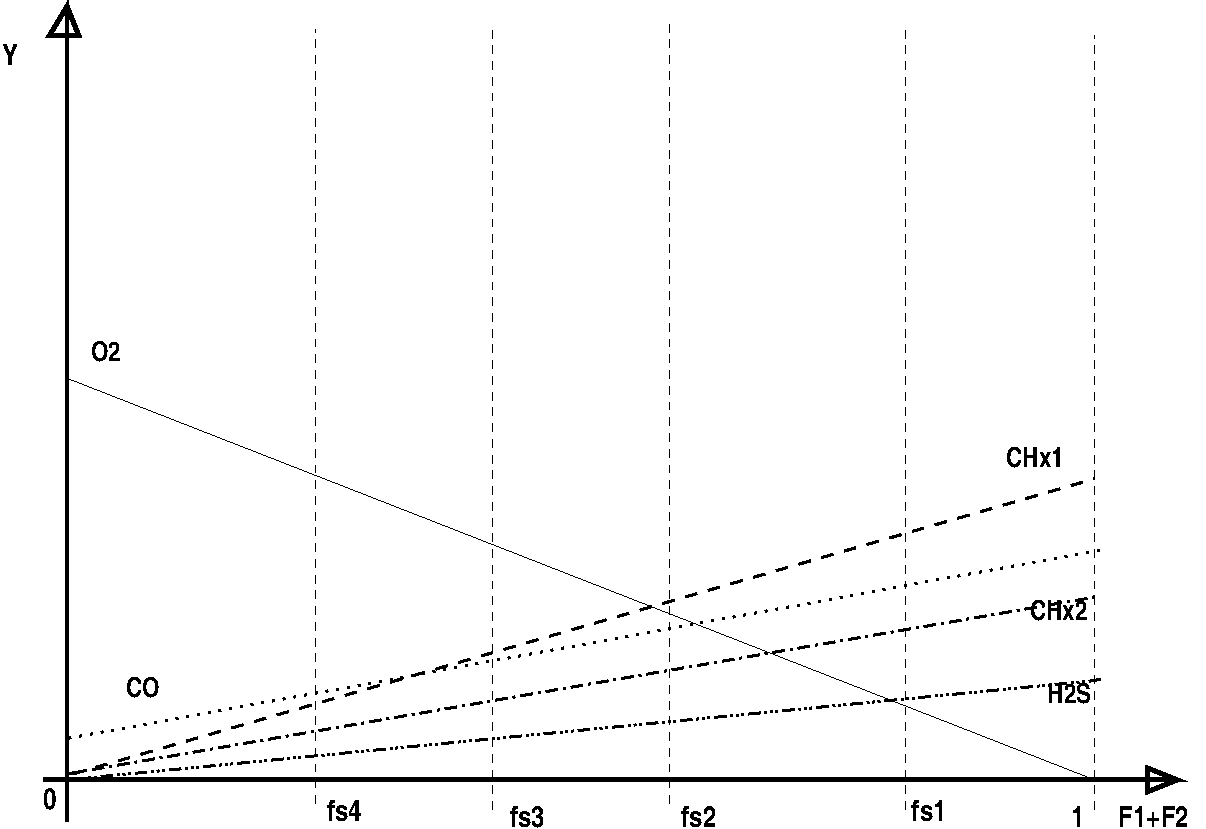
\includegraphics[height=6.2cm]{Yf0}}
\caption{Condensed Fuels before any gas combustion} 
\end{figure}
%========================================
\vspace{0.2in}
Before reaction between gases, only exist species coming from
inlets or interfacial source term : $CO$ in mean local fuel (i.e. $f_1+f_2=1$)
comes from devolatilisation, $CO$ in mean local oxidizer (i.e. $f_1+f_2=0$)
comes from heterogeneous reactions of char.

During pulverised coal combustion, two kinds of volatile matters are considered
and the sketch of concentrations during the three successive reactions is quite
similar.

Every reaction (but, possibly the final conversion of $CO$ to $CO_{2}$) are
supposed to be fast compared to the turbulent mixing, but among these reactions
some can be faster; here, a priority rule to access oxygen is established (the
more eager -for oxygen- the specy, the faster the reaction).\\

The first reaction is a partial dehydrogenation of the light volatile $CH_{x1}$
to form the species caracteristic of heavy volatile $CH_{x2}$: in fs1, all of
$CH_{x1}$ (issued from the low temperature pyrolisis reaction) is converted, and
the $CH_{x2}$ (issued from the high temperature pyrolisis reaction) is
incremented.
\begin{eqnarray}
CH_{x1} + \displaystyle\frac{x1-x2}{4} O_{2} &\Rightarrow& CH_{x2} + \frac{x1-x2}{2} H_{2}O
\end{eqnarray}
%========================================
\begin{figure}[h]
\centerline{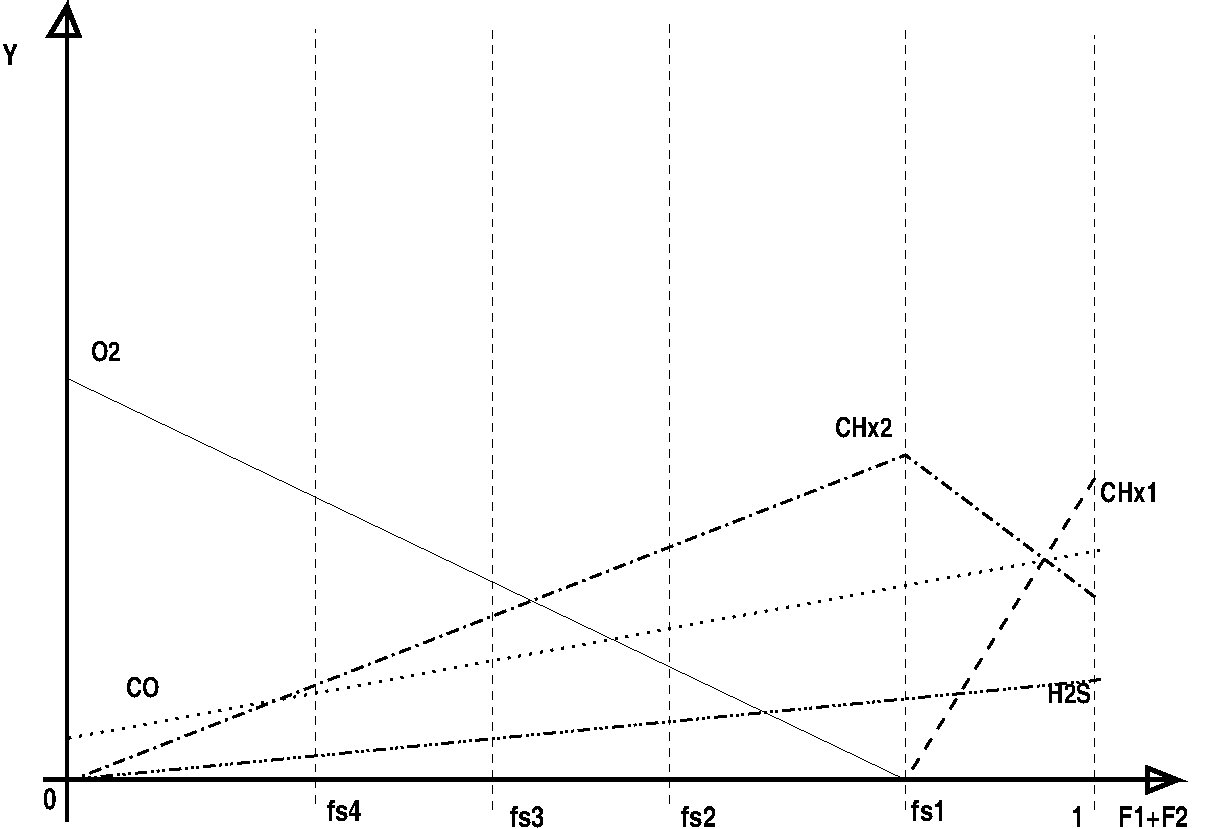
\includegraphics[height=6cm]{Yf1}}
\caption{Condensed Fuels after hydrocarbons conversion} 
\end{figure}
%========================================
 
The oxygen and the hydrocarbon vapor have linear concentrations in f(1+2) on [0,
1]. As long as the stoechiometry of the reaction is known, a simple equation
allows to determine fs2 the stoechiometric point for the second reaction
({\small where both oxygen and hydrocarbon vanish}). The second reaction is the
conversion of some hydrocarbon vapor to carbon monixide and water vapor ({\small
  not plotted in an optimistic attempt to lighten the sketch}).
\begin{eqnarray}
CH_{x2} + \displaystyle \frac{2+x2}{4} O_{2} &\Rightarrow& CO + \frac{x}{2} H_{2}O 
\end{eqnarray}
%========================================
\begin{figure}[h!]
\centerline{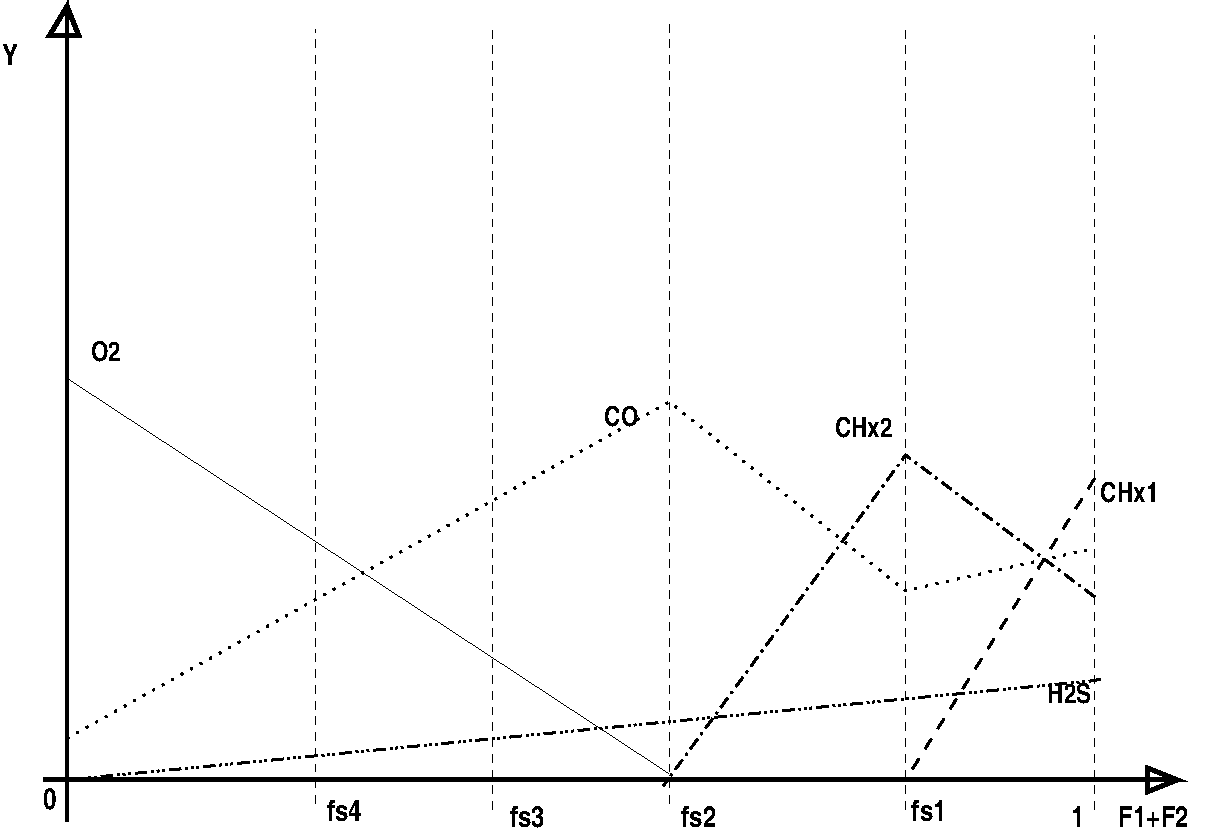
\includegraphics[height=6cm]{Yf2}}
\caption{Condensed Fuels after hydrocarbons oxidation}
\end{figure}
%========================================

Then the rich area can't undergo any reaction (no oxygen available) if the PDF(f) is not zero before Fs2, then some $CH_{x}$ is unburnt.\\
Some $H_{2}S$ can be converted to $SO_{2}$, the carbon monoxide existing between
fs2 and 1 is protected from oxidation (the two first reactions have destroyed
the free oxygen). Like previously, oxygen and hydrogen sulphide have
concentrations linear in f on [0,fs2] as long as the stoechiometry of the
reaction is known, a simple equation allows to determine fs3 the stoechiometric
point for the third reaction (where both oxygen and hydrogen sulphide vanish).
\begin{eqnarray}
H_{2}S + \displaystyle\frac{3}{2} O_{2} &\Rightarrow& SO_{2} + H_{2}O 
\end{eqnarray}
%========================================
\begin{figure}[h!]
\centerline{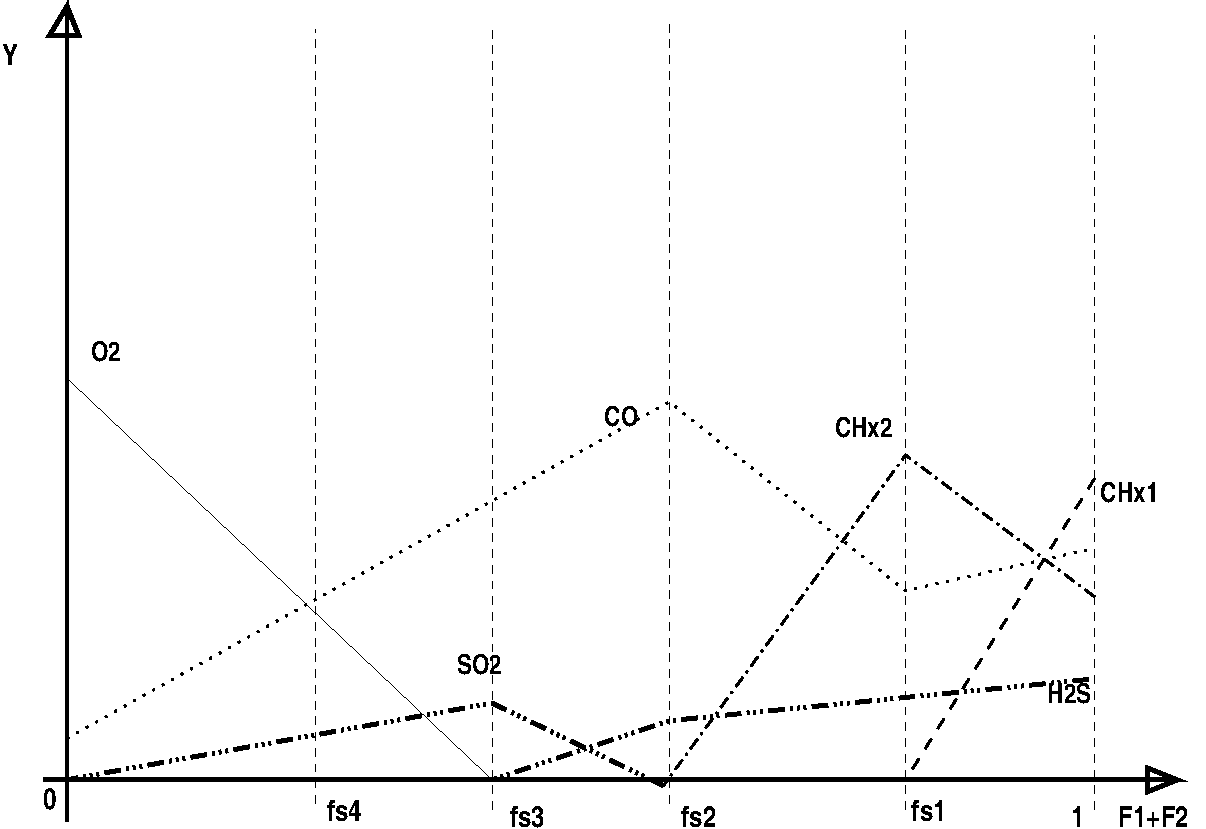
\includegraphics[height=6.2cm]{Yf3}}
\caption{Condensed fuels after H2S oxidation}
\end{figure}
%========================================

If the final conversion of carbon monoxide to carbon dioxide is assumed fast
(with respect to variance dissipation) a last reaction is taken in account:
\begin{eqnarray}
CO + \displaystyle \frac{1}{2} O_{2} &\Rightarrow& CO_{2}
\end{eqnarray}
%========================================
\begin{figure}[h!]
\centerline{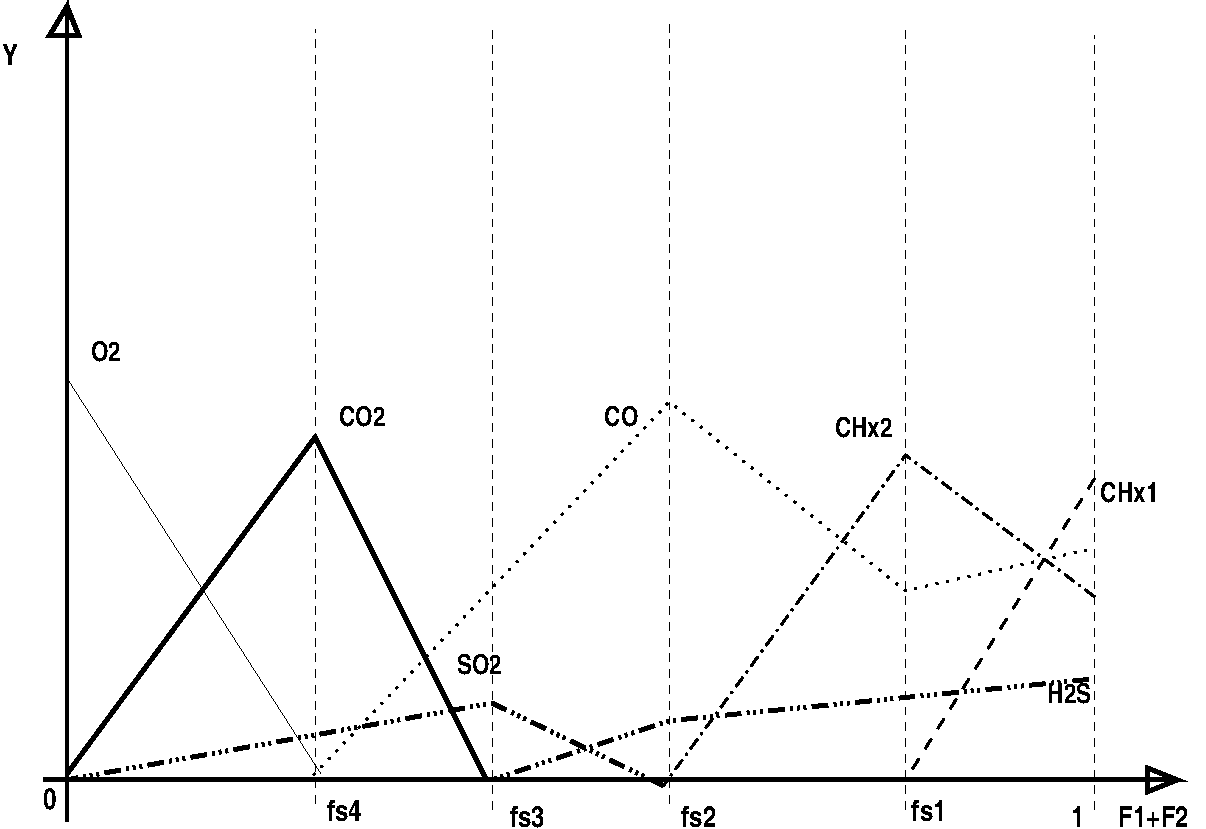
\includegraphics[height=6cm]{Yf4}}
\caption{Condensed Fuels after final oxidation of CO}
\end{figure}
%========================================

Comparisons of the PDF rectangle hedges [$f_{\mbox{\scriptsize deb}} ,
f_{\mbox{\scriptsize fin}}$] and remarkable composition points $[0,
f_{\displaystyle s4}, f_{\displaystyle s3},$ $f_{\displaystyle s2},
f_{\displaystyle s1}, 1]$ allows a simple integration : 1) Dirac's peak
intensity are used to weight composition at boundaries, 2) the piece linear part
is integrated with analytical formulae on each band :
 
%==================
\begin{enumerate}
\item rich range, here existing species with the higher calorific value : \\
  \hspace{0.25cm}$CH_{x}$ (in fuel case) or $CH_{x2}$ (in coal case):
  $[\max(f_{\mbox{\scriptsize deb}},f_{\displaystyle s1}) ;
  \min(f_{\mbox{\scriptsize end}},1)]$
\item upper-middle range $CH_{x1}$ conversion : $[\max(f_{\mbox{\scriptsize
      deb}},f_{\displaystyle s2} ); \min (f_{\mbox{\scriptsize
      end}},f_{\displaystyle s1})]$
\item middle range $H_{2}S$ conversion : $[\max(f_{\mbox{\scriptsize
      deb}},f_{\displaystyle s3} ); \min (f_{\mbox{\scriptsize
      end}},f_{\displaystyle s2})]$
\item working range, carbon monoxide consumption frees enthalpy :
  $[\max(f_{\mbox{\scriptsize deb}},f_{\displaystyle s4} ); \min
  (f_{\mbox{\scriptsize end}},f_{\displaystyle s3})]$
\item poor range, only products and oxidisers : $[\min(f_{\mbox{\scriptsize
      deb}},f_{\displaystyle s4} ); \min (f_{\mbox{\scriptsize
      end}},f_{\displaystyle s4})]$
\end{enumerate}
%==================
For each band (eg. [$f_{\displaystyle si} , f_{\displaystyle sj}$])
concentrations can be written :
\begin{eqnarray}
%---------------
  \displaystyle Y_e & = & Y_{e}(f_{\displaystyle si}) + \frac{f-f_{\displaystyle si}}{f_{\displaystyle sj}-f_{\displaystyle si}} .~ \left( Y_{e}(f_{\displaystyle sj})-Y_{e}(f_{\displaystyle si}) \right) 
%---------------
\end{eqnarray}
Integration on the band [b1 , b2] (obviously $b1 \geq f_{si} \quad \text{and}
\quad b2 \leq f_{sj}$) gives the increment:
\begin{eqnarray}
%---------------
  \displaystyle Y_{e} & := & Y_e + h_{\mbox{\scriptsize \textsc{rec}}}~(b2-b1)  .  \left[ \frac{Y_{e}(f_{si}).~f_{sj}-Y_{e}(f_{sj}).~f_{si}}{f_{sj}-f_{si}}
    \displaystyle                                  +         \frac{Y_{e}(f_{sj})-Y_{e}(f_{si})}{f_{sj}-f_{si}}.~\frac{b1+b2}{2} \right] \qquad
%---------------
\end{eqnarray}
where $h_{\mbox{\scriptsize \textsc{rec}}}$ is the height of the PDF's
rectangle.

%========================================
\section*{Specification of pyrolysis}
%========================================

Coal is currently known by its proximate and ultimate analysis. Ultimate analysis of char can be known or assumed pure carbone.
The point is to determine the amount of volatile matter and their composition ;
the following assumptions are every time done :
%==================
\begin{enumerate}
\item sulphur is released as hydrogen sulphide ($H_{2}S$),
\item nitrogen is released both in HCN and $NH_{3}$, with a ratio which is an user's prescription
\end{enumerate}
%==================

Three ways are available :
%==================
\begin{enumerate}

\item The volatile matter content determined during the proximate analysis is
  supposed to be representative of Y1 selectivity in volatile of the first
  reaction (Kobayashi description involves two parallel reactions, the first has
  a low activation energy and produces ligth volatile matter, the second one has
  a high activation energy and produces heavy volatile matter). Oxygen is
  released as carbon monoxide. No water steam (linked water) among volatile
  matter. So the formulae for the mean hydrocarbon is determined as x1 in
  $CH_{x1}$. The heavy, unsaturated, volatile issued from the second reaction
  are caracterised by $x2$ as an half of $x1$ ; with the same assumption for
  oxygen, Y2 can be computed. User has to check for $x1$ and $x2$ likelihood
  (between 1 and 4).
\item When the proximate analysis is not known, $x1$ is assumed to be equal to
  four (methane is a fairly good model for light volatiles) and $x2$ is assumed
  to be equal to 2 (ethylene and other species with double bound are good models
  for unsaturated species), then selectivites $Y_1$ and $Y_2$ can be deduced
  \ldots and checked (under one).
\item Large amount of oxygen appears in the ultimate analysis of biomass and low
  rank coal (lignite or peat) then linked or bounded water is released during
  pyrolisis (a chemical mechanism taking place at higher temperature than the
  physical drying which releases the "free" water). In this case, an extra
  parameter have to be determined (number of water molecules released during
  pyrolisis), so the user may stipulate both x (in the formulae for hydrocarbon
  $CH_{x}$, as previously 4 and 2 respectively) and Y (the selectivity in
  volatile matter, the proximate analysis set $Y_1$ and $Y_2$ is assumed from
  empirical criterion, e.g. $(1+Y_1)/2$).

\end{enumerate}
%==================

Detail of computation.\\
From ultimate analysis of coal (or heavy fuel oil) and char (if ultimate
analysis of char is lacking, the pure carbon assumption is welcome), global
formulae for the "monomer" (refering to one carbon, so ch...cs and kh...ks are
easy to compute) can be deducted. Then, the reaction (pyrolisis and / or
evaporation) transforming the original fuel in a mixture of gaseous ones and
residual char can be summarized as:
\begin{eqnarray}
%---------------
CH_{ch}O_{co}N_{cn}S_{cs} & \Rightarrow & a . CH_{x} + b . CO + c . H_{2}O + d . H_{2}S + e . HCN + f . NH_{3} \nonumber \\
                          &             & + (1-a-b-e) . CH_{kh}O_{ko}N_{kn}S_{ks}
%---------------
\end{eqnarray} 

The stoechiometric coefficient for char monomer beeing deducted from Carbon
conservation, five equation can be written : four for the conservation of
elements ( H, O, N, S) and one defines the gas selectivity.
\begin{eqnarray}
%---------------
  \text{Hydrogen budget  } \quad ch &=& a.x + 2.c + 2.d + e + 3.f +(1-a-b-e).kh \nonumber \\
  \text{Oxygen budget    } \quad co &=& b + c + (1-a-b-e) . ko \nonumber \\
  \text{Nitrogen budget  } \quad cn &=& e + f + (1-a-b-e).kn \nonumber \\
  \text{Sulphur budget   } \quad cs &=& d + (1-a-b-e) .ks \nonumber \\
  \text{mass ratio of gases or selectivity} \nonumber \\
  a.(12+x) + b.28 +c.18+d.34+e.27+f.17 &=& Y .(12+ch+16.co+14.cn+32.cs)
\end{eqnarray}
But, eight unknown are involved (a, b, c, d, e, f, x, Y), so three extra
conditions are needed to solve the linear system (if ax is considered an
auxiliary unknown in place of x) :
%==================
\begin{enumerate}

\item User assumes the repartition between nitrogenated species by fixing
  reference numbers ei and fi. The equation $ei.f-f_i.e=0$ can be added to the
  system.
\item if the proximate analysis can be used to determine the ratio of gases
  issued from an high rank coal or fuel, Y is know and c (number of water
  molecules issued from decomposition) can be assumed nil. Equations $Y=Yi$ and
  $c=0$ are added.
\item without relevant information about the selectivity, assumption have to be
  done on x (is the released hydrocarbon saturated or not ?), and c can be again
  assumed nil. Equations $a.x_i-ax = 0$ and $c=0$ are added.
\item oxygenated fuels (biomass, lignin) contains bounded water to be released
  during pyrolisis, so proximate analysis (for Y) and assumption about the kind
  of hydrocarbon (for x) are needed. Equations $a.x_i-ax = 0$ and $Y=Y_i$ are
  added.

\end{enumerate}
%==================
Then a 8 x 8 linear system is defined and can be solved by regular algorithm.
 
%===============================================
\section*{Specification of granulometry}
%===============================================

User has to choose the initial diameter of different classes and the sharing out
of the inlet flow. The distribution is often known by some diameters (quantile
or sieves) from which parameters of an assumed Rossin-Ramler law can be fitted
(least squares). Then choosing the number of classes and flow partition allows
computation of the initial diameter of each class. Obviously, the finest
particles or droplets are responsible for the ignition and stability of the
flamme and the biggest ones are responsible for unburnt carbon in ash. So two
common descritions are ten classes, each of them with a tenth of the flow, or
five classes with (0.1 , 0.2 , 0.4 , 0.2 , 0.1) of the flow. The second way is
nearly two times cheaper (in computer time) but includes the same extreme
diameters. \\
By definition of the Rossin-Ramler law as used in granulometry, the mass
fraction associated with particles finer than a diameter obeys :
\begin{equation}
  \displaystyle P(\mbox{\small d}_i) = 1-\exp{\left[-\displaystyle\frac{\mbox{\small d}_i}{D_m} ^n \right]}
\end{equation} 
Where, surprinsgly, n is not an integer (but a real) and Dm is not the median
diameter. When only two data are available (pass through two sieves, extreme
deciles or quartiles) the determination of Rossin-Ramler law parameters is
direct :
\begin{eqnarray}
  \displaystyle P(\mbox{\small d}_1) &=& 1-\exp\left[-\frac{\mbox{\small d}_1}{D_m}^n\right] \label{Eqs_log_001} \\
  \displaystyle P(\mbox{\small d}_2) &=& 1-\exp\left[-\frac{\mbox{\small d}_2}{D_m}^n\right] \label{Eqs_log_002}
\end{eqnarray}
The logarithm forms of (Eqs.~\ref{Eqs_log_001}-\ref{Eqs_log_002}) are the
following expressions:
\begin{eqnarray}
  \displaystyle \left(\frac{\mbox{\small d}_1}{D_m} \right)^n &=& - \log(1-P_1) \label{Eqs_log_003} \\
  \displaystyle \left(\frac{\mbox{\small d}_2}{D_m} \right)^n &=& - \log(1-P_2) \label{Eqs_log_004} 
\end{eqnarray}
The logarithm forms of (Eqs. ~\ref{Eqs_log_003}-\ref{Eqs_log_004})
are:\vspace{-0.1in}
\begin{eqnarray}
  \displaystyle n . \left[~ \log(\mbox{\small d}_1)-\log(D_m)~\right] &=& \log[~-\log(1-P_1)~] \label{Eqs_log_005} \\
  \displaystyle n . \left[~ \log(\mbox{\small d}_2)-\log(D_m)~\right] &=& \log[~-\log(1-P_2)~] \label{Eqs_log_006}
\end{eqnarray}\vspace{-0.1in}
Using the expressions (Eqs.~\ref{Eqs_log_005}-\ref{Eqs_log_006}) we obtain:\vspace{-0.1in}
\begin{eqnarray}
n &=& \frac{\log \left[\displaystyle\frac{ \log(1-P_1)}{\log(1-P_2)}\right]}{\displaystyle\log\left[\frac{\mbox{\small d}_1}{\mbox{\small d}_2} \right]} 
\end{eqnarray}
and~ $D_m$ is easily deduced.

When more data are available, the second logarithm relation gives a cloud of
couple ($\log(\mbox{\small d}_i)$ , $\log[~-\log(1-P_i)~]$ ) among which a
linear fit is looked for ($n, n.\log(D_m)$):
\begin{eqnarray}
  \displaystyle n . \log(\mbox{\small d}_i)- \left[~n.\log(D_m)~\right] &=& \log[~-\log(1-P_i)~] \label{Eqs_log_007}\\
  a.x_i + b &=& y_i \nonumber
\end{eqnarray}
Least square formulae are then used ... after a data transformation (two
logarithm) relevant for the distance.
\begin{eqnarray}
a &=& \frac{N \sum x_i.y_i - \sum x_i . \sum y_i}{N.\sum x_i^2 - \left( \sum x_i\right)^2} \label{Eqs_log_008}
\end{eqnarray}
Where N is the number of data.
\begin{eqnarray}
n &=& \frac{N \sum \log[\mbox{\small d}_i].\log[~-\log(1-P_i)~] - \sum \log(\mbox{\small d}_i) . \sum \log[~-\log(1-P_i)~]}{N.\sum \log(\mbox{\small d}_i)^2 - \left( \sum \log(\mbox{\small d}_i)\right)^2} \label{Eqs_log_009} \\
b &=& \frac{\sum y_i . \sum x_i^2 - \sum x_i . \sum x_i.y_i }{N.\sum x_i^2 - \left( \sum x_i\right)^2} \label{Eqs_log_010} \\ 
-n.\log(D_m) &=& \frac{\sum \log[~-\log(1-P_i)~] . \sum \log(\mbox{\small d}_i)^2 - \sum \log(\mbox{\small d}_i) . \sum \log(\mbox{\small d}_i).\log[~-\log(1-P_i)~] }{N.\sum \log(\mbox{\small d}_i)^2 - \left( \sum \log(\mbox{\small d}_i)\right)^2}\qquad \qquad\label{Eqs_log_011}
\end{eqnarray}
After this laborious identification of parameters (done by Excel), the
determination of the mean diameter of each mass class is obtained from the
definition of the rossin-Ramler law :
\begin{equation}
\displaystyle \mbox{\small d}_i = D_m ~ \left[-\log(1-P_i) \right]^{\left(\textstyle \frac{1}{n} \right)} \label{Eqs_log_012}
\end{equation} 
As an example, if the user chooses the (recommended) sharing out $\left[0.1 , 0.2 , 0.4 , 0.2, 0.1 \right]$, the corresponding diameter are deduced from the \textit{mean cumulated mass} as:
\begin{eqnarray}
\Delta_{1} = 0.1 \text{ ; } \Sigma_{1} = 0.1 \quad  ; \quad 1-MCM_{1}=~~~~1~~-~~\frac{0.1}{2}~=0.95 &\Rightarrow&
           \mbox{\small d}_1 = Dm ~ \left[~ -\log(0.95) ~\right]^{\left(\textstyle \frac{1}{n}\right)} \nonumber \\
\Delta_{2} = 0.2 \text{ ; } \Sigma_{2} = 0.3 \quad  ; \quad 1-MCM_{2}=1-\frac{0.1+0.3}{2}= 0.80 &\Rightarrow& 
           \mbox{\small d}_2 = Dm ~ \left[~ -\log(0.80) ~\right]^{\left(\textstyle \frac{1}{n}\right)} \nonumber \\
\Delta_{3} = 0.4 \text{ ; } \Sigma_{3} = 0.7 \quad  ; \quad 1-MCM_{3}=1-\frac{0.3+0.7}{2}= 0.50 &\Rightarrow& 
           \mbox{\small d}_3 = Dm ~ \left[~ -\log(0.50) ~\right]^{\left(\textstyle \frac{1}{n}\right)} \qquad \qquad \\
	   %\label{Eqs_log_13} \\
\Delta_{4} = 0.2 \text{ ; } \Sigma_{4} = 0.9 \quad  ; \quad 1-MCM_{4}=1-\frac{0.7+0.9}{2}= 0.20 &\Rightarrow& 
           \mbox{\small d}_4 = Dm ~ \left[~ -\log(0.20) ~\right]^{\textstyle\left( \frac{1}{n}\right)} \nonumber \\
\Delta_{5} = 0.1 \text{ ; } \Sigma_{5} = 1.0 \quad  ; \quad 1-MCM_{5}=1-\frac{0.9+1.0}{2}= 0.05 &\Rightarrow& 
           \mbox{\small d}_5 = Dm ~ \left[~ -\log(0.05) ~\right]^{\left(\textstyle \frac{1}{n}\right)} \nonumber
\end{eqnarray}
With such a symetrical mass distribution, the diameter of the central class is the median diameter of the Rossin-Ramler (i.e. half of the mass is contained in more tiny particles).

%===============================================
\section*{Special attention paid to variance}
%===============================================

With the gaz phase combustion model, everything is quite simple : two variables
are relevant, the mean and the variance of the mixture fraction. With the two
phase combustion model, a lot of mixture fractions are defined and the pdf model
is constructed for the sum of the two mixture fractions related with
volatiles. So the source term related with the square of the gradient of the
mean can't be computed as for regular variance (the \fort{gradcel} subroutine is
called for the sum).

In \CS~ homogeneous two phase flow, only one velocity is defined, and all
variables refer to the bulk (sum of gaseous and condensed phase), but the pdf
has to be defined only in the gas phase. So phasic mean and variance have to be
defined, with the special difficulties of variables undefined in the condensed
phase ($f_i$ is a mixture fraction in gas on mixture: kg coming from $i / kg$ of
mixture):
\begin{eqnarray}
\widetilde{f} = X_{1}.f^{*} + X_{2}.0 \quad &\Rightarrow& \quad f^{*} = \frac{\tilde f}{1-X_{2}}                        \label{Eqs_var_001}\\
\widetilde{f}^{2} = X_{1}.\left( f^{*2} + f''^{2*} \right)+ X_{2}.0 \quad &\Rightarrow& \quad f^{*2} + f''^{2*} = \frac{\widetilde f^{2}}{1-X_{2}}                                                                                                                                          \label{Eqs_va_002} \\
f''^{2*} &=& \frac{\widetilde f^{2}}{1-X_{2}} - \left( \frac{\tilde f}{1-X_{2}}\right)^{\textstyle 2}                   \label{Eqs_var_003}\\
f''^{2*} &=& \frac{(\tilde f)^{2} + \widetilde f''^{2}}{1-X_{2}} - \left( \frac{\tilde f}{1-X_{2}}\right)^{\textstyle2} \label{Eqs_var_004}\\
f''^{2*} &=& \frac{\widetilde f''^{2}}{1-X_{2}} -  \frac{X_{2}.(\tilde f)^{2}}{(1-X_{2})^{2}}                           \label{Eqs_var_005}\\
f''^{2*} &=& \frac{\widetilde f''^{2} - \frac{X_{2}}{X_{1}}.(\tilde f)^{2} }{X_{1}}                                     \label{Eqs_var_006}
\end{eqnarray}
Only this phasic variance (the part of the variance in the gas phase)
is able to dissipate : so, the second part of the source term for variance has
to be modified.\\
Last but not least, mass flux crossing the interface (pyrolisis fluxes) are made
of pure volatile matter and mixes with a gas at any value of mixture fraction
mean. So the interfacial flux constitutes a source term for the mean and for the
variance, following Escaich \cite{1}, the closure would be :
\begin{equation}
\displaystyle S_{\widetilde{.''^2}} = \Gamma . \left( f_{\mbox{\scriptsize\textsc{cl}}} -\tilde f \right) . \left( 2.f_{\Gamma} - f_{\mbox{\scriptsize\textsc{cl}}} - \tilde f \right)
\end{equation}
In which, $\Gamma$ is the mass flux, $f_{\Gamma}$ is the value of the mixture
fraction in the flux (1 for pyrolisis or fuel evaporation),
$f_{\mbox{\scriptsize\textsc{cl}}}$ is the value of the mixture fraction in the
boundary layer ... to be closed by a relevant assumption : from laminar or
turbulent diffusion (to do in \fort{coal\_variance\_source\_term} or
\fort{fuel\_variance\_source\_term}, not available for regular users).\\
With an assumption of laminar diffusion around each particle able to transport
the mass flux :
\begin{equation}
\displaystyle f_{\mbox{\scriptsize\textsc{cl}}} =  1 - (1-\tilde f)\exp \left[\displaystyle \frac{\Gamma}{2 \pi D d \rho}\right]
\end{equation} 
When mass flux is huge, the diffusion can't stay regular around each inclusion :
if the variance is maximal (intermittency assumption), the boundary layer can't
be no more distinguished from the mean, if the variance vanish, the boundary
layer is quiet and made of outing gases :
\begin{equation}
\displaystyle f_{\mbox{\scriptsize\textsc{cl}}} = f_{\Gamma} + (\tilde f  - f_{\Gamma}) ~ \frac{\widetilde f^{''2}}{\tilde f .(1-\tilde f)}
\end{equation} 
This special assumption allows a term source for variance easy to implicit in order to avoid overshoot (the variance have a maximal value related to the mean) :
\begin{equation}
\displaystyle S_{\widetilde ''^{2}} = \Gamma .\left( f_{\Gamma}-\tilde f\right)^{2} ~ \left\{ 1-\left[~ \frac{\widetilde f^{''2}}{\tilde f ~(1-\tilde f)}~\right]^{\textstyle2}\right\}
\end{equation}


%========================================
\section*{NOx}
%========================================

Nitrogen oxides are a key pollutant, an accurate prediction is difficult but the
relative effect of modification (of fuel, of stagging, and so on) is a reachable
goal.
Hereafter, the two main ways of nitrogen oxides formation are supposed to
be thermal NOx (reaction between molecular nitrogen and radical oxygen activated
at the higher temperature) and fuel NOx (resulting from the oxidation of
nitrogen originating from fuel) are described and taken in account in the \CS~
model for diphasic combustion. The third way, resulting of reaction between the
molecular nitrogen and hydrocarbon radicals is assumed negligible in diphasic
combustion ; its contribution is worthy of attention only for gas combustion
(especially in dry
low NOx combustor for gas turbine).\\

\subsection*{Thermal NOx}
In the Zeldovich mechanism, the rate of the key reaction, between molecular
nitrogen and radical oxygen, has a simple expression thanks to an assumption of
equilibrium applied on oxygen dissociation, leading to :
\begin{eqnarray}
 N_{2} + O_{2} &\Rightarrow& 2 ~NO \nonumber \\
 W1_{NO}&=& 3.4\medspace10^{12}  .   \exp \left[\frac{-66\medspace900}{RT}\right].\left[ N_{2} \right] . \left[O_{2}\right]^{1/2}
\end{eqnarray} 
 
This production term has to be evaluated in each fluid particle because it is not
only non linear (with respect to mixture fraction) but submitted to segregation :
the hottest particles are near the stoechiometric point ... where oxygen is
exhausted (and vice versa). As a consequence, simplest approximations, neglecting
covariances, are not satisfaying :\\

\begin{equation}
 \widetilde{W_1}_{NO} \neq k_0  . \exp \left[\frac{E}{R\tilde{T}}\right].\left[ \widetilde{N}_{2} \right].\left[\widetilde{O}_{2}\right]^{1/2}
\end{equation}
Taking in account only the mean temperature, the contribution of hotest fuilds particles disappears and nitrogen oxide formation is under estimated.\\
The source term for thermal NOx has to be integrated following the example of
others turbulents variables (like species mass fractions). In the turbulent
oxydation model, mass fraction of species are known linear piecewise functions,
the oxygen fraction is positive only between the mean local oxidizer and fs3 the
stoechiometric point for the "last" reaction ($H_{2}S$ conversion), the post
conversion of carbon monoxide to carbon dioxide is assumed to result from a
relaxation to the thermodynamical equilibrium computed with mean values. The
stoechiometric point corresponding to this last reaction is no more necessary to
the turbulent computation but for temperature evaluation : as, by now, the mean
local oxidiser includes some carbon monoxide (originating from heterogeneous
reactions involving char), it can't be no more supposed unreactive, assuming a
linear profile for oxygen, and carbon monoxide, between the local mean oxidiser
and the point where hydrocarbon oxidation is finished, the mass fraction in the
local mean oxidizer are auxilliary unknowns the value of which is determinated
by equalizing the transported value for the carbon monoxide (which involves the
effect of relaxation to equilibrium) and its integrated value (taking in account
the local pdf).
   

%========================================
\begin{figure}[h!]
\centerline{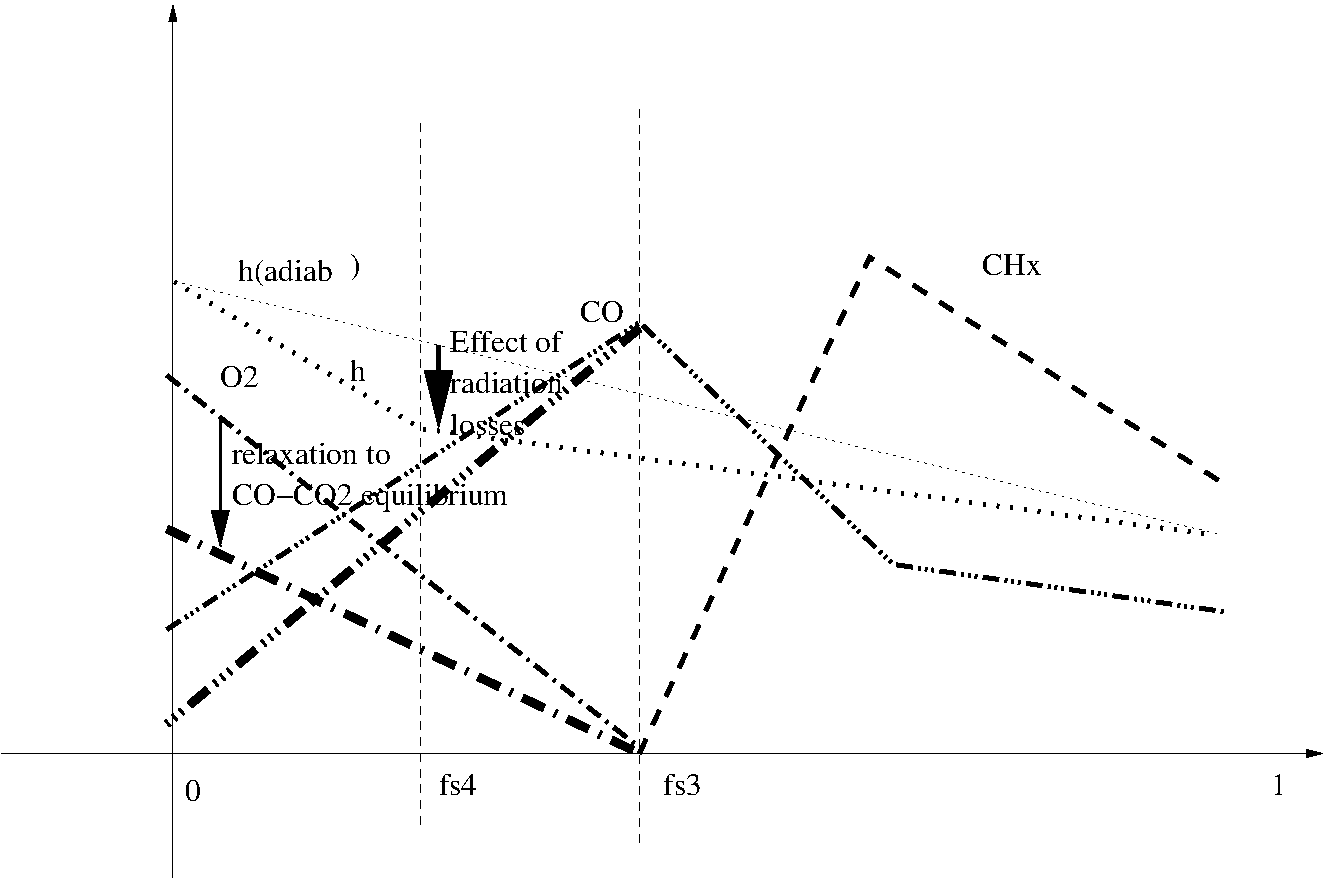
\includegraphics[height=6cm]{TONOx}}
\caption{Mass fractions of reactive species, turbulent reaction then kinetical relaxation, enthalpy with radiation losses}
\end{figure}
%========================================

Assuming the entalpy piecewise linear with the enthalpy in fs4 considered as an
auxilliairy unknown, which can be determined by equalizing the integrated
enthalpy and the transported one (the tranport equation of which includes
radiation losses), then the temperature piecewiselinear with respect to the
mixture fraction, the numerical integration of the source term is now available,
using a regular trapezium method with 200 points (between the pdf's rectangle
begining and the minimum of fs3 and pdf's rectangle end).

\subsection* {Fuel NOx}
The nitrogen included in the organic part of the fuel (can be a significant part
of some biomass, like agricultural residues, oil cake and so on) evolves to
$HCN$. This reducing form of nitrogen can be oxydised either by oxygen or by
nitrogen oxide :

\begin{eqnarray}
HCN + \frac{5}{4}~ O_{2} &\Rightarrow& NO + \frac{1}{2} ~H_{2}O + CO \nonumber \\
 W2_{NO} &=& 3 \medspace10^{12} \exp \left[\frac{- 30\medspace000}{RT}\right].\left[ HCN \right] . \left[O_{2}\right]^{\textstyle b}\\
\left[O_{2}\right] < 0.0025 &;& b = 1 \nonumber \\
0.0025 < \left[O_{2}\right] < 0.018 &;& b = \frac{0.018-\left[O_{2}\right]}{0.018-0.0025} \nonumber \\
0.018 < \left[O_{2}\right] &;& b = 0 \nonumber
\end{eqnarray}
In the last case, $NO$ is reduced to nitrogen : the fuel nitrogen contributes to destroy even thermal NO.
\begin{eqnarray}
 HCN + NO + \frac{1}{4}~ O_{2} &\Rightarrow& N_{2} + \frac{1}{2}~ H_{2}O + CO \nonumber \\
 W3_{NO} &=& 1.2 \medspace 10^{10}  .  \exp \left[\frac{-33\medspace500}{RT}\right].\left[ HCN \right] . \left[NO\right]
\end{eqnarray} 
\

%=================================
%=================================
%\clearpage

%=================================
\section*[Conservation Equations]{Conservation Equations for two phase flow combustion}
%=================================

%%%%%%%%%%%%%%%%%%%%%%%%%%%%%%%%%%%%%%%%%%%%%%%%%%%%%%%%%%%%%%%%%%%%%%%%%%%%%%%%%%%%%%%%%%%%%%%%%%%%%%%%%%%%%%%%%%%%%%%%%%%%%%%%%%%%%%%%%%%%%%%%% 
The bulk, made of gases and particles, is assumed to be modeled with only one pressure and velocity. The slipping velocitiy between particles 
and gases is supposed negligible compared to this mean velocity.
Scalars for the bulk are:
%%%%%%%%%%%%%%%%%%%%%%%%%%%%%%%%%%%%%%%%%%%%%%%%%%%%%%%%%%%%%%%%%%%%%%%%%%%%%%%%%%%%%%%%%%%%%%%%%%%%%%%%%%%%%%%%%%%%%%%%%%%%%%%%%%%%%%%%%%%%%%%%% 
\vspace{0.5cm}
%==================
\begin{itemize}
  \item Bulk density 
     \begin{equation} 
     %---------------
        \rho_{m} = \alpha_{1}\rho_{1} + \alpha_{2}\rho_{2}
     %---------------
     \end{equation} 
     %\nomenclature{$\rho _m$}{bulk density [$kg/m^3$]}
     %\nomenclature{$ \alpha _i$}{mass fraction of phase k}

  \item Bulk velocity 
     \begin{equation} 
     %---------------
       U_{m} = \frac{ \alpha_{1}\rho_{1} U_{m} 
                    + \alpha_{2}\rho_{2} U_{m} }{\rho_{m}}
     %---------------
     \end{equation}
     %\nomenclature{$U_m$}{bulk velocity [$m/s$]}

  \item Bulk enthalpy 
     \begin{equation} 
     %---------------
        H_{m} = \frac{ \alpha_{1}\rho_{1}.H_{1} 
                     + \sum_{1}^{npar}\alpha_{2,ipar}\rho_{2}.H_{2,ipar} }{\rho_{m}}
     %---------------
     \end{equation} 
     %\nomenclature{$H_m$}{bulk enthalpy [$J/kg$]}

  \item Bulk pressure 
     \begin{equation} 
     %---------------
       P_{m} = P_{1}
     %---------------
     \end{equation}
     %\nomenclature{P}{pressure [Pa]}
\end{itemize}
%===========

Mass fractions of gaseous medium ($Y_{1}^{*}$) and of particles are defined by:
\begin{eqnarray}
%---------------
  Y_{1}^{*} &=& \frac{\alpha_{1}\rho_{1}}{\rho_{m}} \nonumber\\
  Y_{2}^{*} &=& \frac{\sum_{1}^{npar}\alpha_{2,ipar} \rho_{2}}{\rho_{m}} 
%---------------
\end{eqnarray}
%\nomenclature{$Y_i$}{mass fraction of constituant $i$}

So budget equations for the bulk can be written as following
(\ref{Eq_001}-\ref{Eq_003}):

\begin{eqnarray}
%---------------
\displaystyle  \frac{\partial}{\partial t    } \rho_{m}
\displaystyle +\frac{\partial}{\partial x_{j}} (\rho_{m}U_{m,j}) & = & 0                                                                                                 \label{Eq_001} \\ 
\displaystyle  \frac{\partial}{\partial t    } (\rho_{m}U_{m,i})
\displaystyle +\frac{\partial}{\partial x_{j}} (\rho_{m}U_{m,i}U_{m,j})
\displaystyle                                                    & = &  \frac{\partial}{\partial x_{j}} \left[ 
\displaystyle                                                                       \rho_{m}~D_{m}^{t}\left( \frac{\partial U_{m,i}}{\partial x_{j}}
\displaystyle                                                                                          +\frac{\partial U_{m,i}}{\partial x_{j}} \right) \right]          \nonumber \\
\displaystyle                                                    & + &  \frac{\partial}{\partial x_{j}} \left[        
\displaystyle                                                                                          -\frac{2}{3}\delta_{ij}\left(  q_{m}^{2}
\displaystyle                                                                                          +D_{m}^{t}\frac{\partial U_{m,l}}{\partial x_{l}}\right) \right]
\displaystyle                                                                                          -\frac{\partial P_{m}}{\partial x_{i}}+\rho_{m}g_{i}    \quad           \label{Eq_002} \\
\displaystyle  \frac{\partial}{\partial t    } (\rho_{m} H_{m})
\displaystyle +\frac{\partial}{\partial x_{j}} (\rho_{m}U_{m,j}H_{m})
\displaystyle                                                    & = & \frac{\partial}{\partial x_{j}} (\rho_{m}D_{m}^{t} \frac{\partial H_{m}}{\partial x_{j}}) + S_{m,R}\label{Eq_003}
%---------------
\end{eqnarray}
%\nomenclature{$t$}{time [s]}

%%%%%%%%%%%%%%%%%%%%%%%%%%%%%%%%%%%%%%%%%%%%%%%%%%%%%%%%%%%%%%%%%%%%%%%%%%%%%%%%%%%%%%%%%%%%%%%%%%%%%%%%%%%%%%%%%%%%%%%%%%%%%%%%%%%%%%%%%%%%%%%%% 
With the (velocity) homogeneity assumption, mainly budget equation for bulk
caracteristic are pertinent. So transport equation for the scalar $\Phi_{k}$,
where k is the phase, can be written:
%%%%%%%%%%%%%%%%%%%%%%%%%%%%%%%%%%%%%%%%%%%%%%%%%%%%%%%%%%%%%%%%%%%%%%%%%%%%%%%%%%%%%%%%%%%%%%%%%%%%%%%%%%%%%%%%%%%%%%%%%%%%%%%%%%%%%%%%%%%%%%%%% 

\begin{equation}
%---------------
  \frac{\partial}{\partial t    } (\rho_{m} Y_{k}^{*}\Phi_{k})
 +\frac{\partial}{\partial x_{j}} (\rho_{m} U_{m,j} Y_{k}^{*} \Phi_{k})
              = \frac{\partial}{\partial x_{j}} 
                       (\rho_{m}D_{m}^{t} \frac{\partial Y_{k}^{*} \Phi_{k}}{\partial x_{j}})
               +S_{\Phi_{k}}+\Gamma_{\Phi_{k}}
%---------------
\end{equation}


\subsubsection*{Bulk enthalpy: $H_{m}$ }
%=======================================

Budget equation for the specific enthalpy of the mixture (gas + particles)
admits only one source term for radiative effects
$S_{m,\mbox{\scriptsize\textsc{r}}}$:
\begin{equation}
%---------------
    S_{m,\mbox{\scriptsize\textsc{r}}}= S_{1,\mbox{\scriptsize\textsc{r}}}+ S_{2,\mbox{\scriptsize\textsc{r}}}
%---------------
\end{equation}
With contributions of each phase liable to be described by different models (eg
: wide band for gases, black body for particles).

\subsubsection*{Particles enthalpy: $Y_{2}^{*}H_{2}$ }
%=====================================================

Enthalpy of droplets (J in particles/kg bulk) is the product of solid phase mass
fraction (kg liq/kg bulk) by the specific enthalpy of solid (kg solid/kg
bulk). So the budget equation for liquid enthalpy has six source terms :
\begin{eqnarray}
\Pi_{2}^{'}+S_{2,\mbox{\scriptsize\textsc{r}}}-\Gamma_{\mbox{\small evap}}H_{\mbox{\small H2O,vap}}(T_{2}) & - & \Gamma_{\mbox{\small devol}_1}H_{\mbox{\scriptsize MV1}}(T_{2})\quad-\quad \Gamma_{\mbox{\small devol}_2}H_{\mbox{\scriptsize MV2}}(T_{2}) \nonumber\\
                                                   & + &\Gamma_{\mbox{\small het}}\left( \frac{M_{\mbox{\small O}}}{M_{\mbox{\small C}}}H_{\mbox{\small O}_{2}}(T_{1})~ - ~\frac{M_{\mbox{\small CO}}}{M_{\mbox{\small C}}}H_{\mbox{\small CO}}(T_{2})\right) 
\end{eqnarray}
with
%==================
\begin{itemize}
  \item $\Pi_{2}^{'}$: heat flux between phases,
  \item $S_{2,\mbox{\scriptsize\textsc{r}}}$: radiative source term for droplets,
  \item $\Gamma_{\mbox{\small evap}}H_{\mbox{\small H2O,vap}}(T_{2})$ the vapor
    flux leaves at particle temperature ($H_{\mbox{\small vap}}$ includes latent
    heat),
  \item $\Gamma_{\mbox{\small dvol1}}H_{\mbox{\scriptsize MV1}}(T_{2})$ the
    light volatile matter flux leaves at particle temperature ($H_{\mbox{\small
        vap}}$ includes latent heat),
  \item $\Gamma_{\mbox{\small dvol2}}H_{\mbox{\scriptsize MV2}}(T_{2})$ the
    heavy volatile matter flux leaves at particle temperature ($H_{\mbox{\small
        vap}}$ includes latent heat),
  \item $\Gamma_{het}(...)$ heterogenous combustion induces reciprocal mass
    flux: oxygen arriving at gas temperature and carbon monoxide leaving at char
    particle one.
\end{itemize}
%==================

\subsubsection*{Dispersed phase mass fraction: $Y_{2}^{*}$}
%==========================================================

%%%%%%%%%%%%%%%%%%%%%%%%%%%%%%%%%%%%%%%%%%%%%%%%%%%%%%%%%%%%%%%%%%%%%%%%%%%%%%%%%%%%%%%%%%%%%%%%%%%%%%%%%%%%%%%%%%%%%%%%%%%%%%%%%%%%%%%%%%%%%%%%% 
In budget equation for the mass fraction of the dispersed phase (first droplets,
then char particles, at last ashes) the source terms are interfacial mass fluxes
(first evaporation, then net flux for heterogeneous combustion):

\begin{equation}
%---------------
     -\Gamma_{\mbox{\small evap}}-\Gamma_{\mbox{\small het}}-\Gamma_{\mbox{\small gas,H2O}}-\Gamma_{\mbox{\small gas,CO2}}
%---------------
\end{equation}
The fuel is described by only one amount (for each diameter class) under a
percentile of the initial mass (or diameter), the droplet is supposed to become
a char particle. Under a more little diameter the particle is supposed to become
an ash particle (inert).

\begin{equation}
%---------------
     -\Gamma_{\mbox{\small pyrol}1}-\Gamma_{\mbox{\small pyrol}2}-\Gamma_{\mbox{\small het}}-\Gamma_{\mbox{\small gas,H2O}}-\Gamma_{\mbox{\small gas,CO2}}
%---------------
\end{equation}
The coal or biomass particles are described by three mass component : water
(free : available for drying), reactive coal (available for pyrolisis), char
(available for heterogeneous oxidation and gasification). The mass of ash is
computed with respect to the number of particles, initial size and initial
amount of ashes. The sum of these four component is the amount of each class
(initial diameter and kind of coal).
          
\subsubsection*{Number of particles: $N_{p}^{*}$}
%================================================
No source term in the budget equation for number of droplets or solid particles
: a droplet became a particle (eventually a tiny flying ash) but never vanish
(all particles have to get out).

                                
\subsubsection*{Mean of the passive scalar for light volatile: $F_{1}$}  
%======================================================================

This scalar represents the amount of matter released by the first (low
activation energy) pyrolisis reaction. It is a mass fraction of gaseous matter
(in hydrocarbon form or carbon oxide one). So the source term in its budget is
only the pyrolisis mass flux :
%%%%%%%%%%%%%%%%%%%%%%%%%%%%%%%%%%%%%%%%%%%%%%%%%%%%%%%%%%%%%%%%%%%%%%%%%%%%%%%%%%%%%%%%%%%%%%%%%%%%%%%%%%%%%%%%%%%%%%%%%%%%%%%%%%%%%%%%%%%%%%%%% 
\begin{equation}
    \Gamma _{\mbox{\small pyrol}}
\end{equation}
\subsubsection*{Mean of the passive scalar for heavy volatile: $F_{2}$}  
%======================================================================

This scalar represents the amount of matter which has leaved the droplet as fuel
vapour or the particle by the second (high activation energy reaction), whatever
it happens after. It's a mass fraction of gaseous matter (in hydrocarbon form or
carbon oxide ones). So the source term in its budget is only evaporation or
pyrolisis mass flux :
%%%%%%%%%%%%%%%%%%%%%%%%%%%%%%%%%%%%%%%%%%%%%%%%%%%%%%%%%%%%%%%%%%%%%%%%%%%%%%%%%%%%%%%%%%%%%%%%%%%%%%%%%%%%%%%%%%%%%%%%%%%%%%%%%%%%%%%%%%%%%%%%% 
\begin{equation}
%---------------
    \Gamma_{\mbox{\small pyrol1}} \quad \text{or} \quad \Gamma_{\mbox{\small evap}}
%---------------
\end{equation}     

\subsubsection*{Mean of the passive scalar for oxidizers: $F_{3}$ to $F_{5}$}  
%========================================================================

Budget equation for the three different oxidizers taken in account don't have
any source term.
\subsubsection*{Mean of the passive scalar for steam from drying: $F_{6}$}  
%========================================================================
 
Budget equation for the water steam issued from drying of coal or biomass has
one source term :
\begin{equation}
%---------------
    \Gamma_{\mbox{\small dry}} 
%---------------
\end{equation} 

                                              
\subsubsection*{Mean of the passive scalar for carbon from char oxidation: $F_{7}$}  
%========================================================================
  
Budget equation for $F_{7}$ hase for source term the mass flux due to
heterogeneous combustion (mass flux of carbon monoxide minus oxygene mass
flux). As for $F_{1}$, oxidation in the gaseous phase does not modifiy this {\em
  passive} scalar :

\begin{equation}
%---------------
   \Gamma_{\mbox{\small het}}
%---------------
\end{equation}   
         
 \subsubsection*{Mean of the passive scalar for gasification by the carbon dioxide: $F_{8}$}  
 
 Budget equation for $F_{8}$ has for source term the mass flux due to
 heterogeneous combustion (mass flux of carbon monoxide minus oxygene mass
 flux). As for $F_{1}$, oxidation in the gaseous phase does not modifiy this
 {\em passive} scalar:
  
\begin{equation}
%---------------
   \Gamma_{\mbox{\small gas,CO2}}
%---------------
\end{equation}                         

 \subsubsection*{Mean of the passive scalar for gasification by steam: $F_{9}$}  
 
 Budget equation for $F_{9}$ have for one source term the mass flux due to
 heterogeneous combustion (mass flux of carbon monoxide minus oxygene mass
 flux). As for $F_{1}$, oxidation in the gaseous phase does not modifiy this
 {\em passive} scalar:
 
\begin{equation}
%---------------
   \Gamma_{\mbox{\small gas,H2O}}
%---------------
\end{equation}                         

 

%\clearpage


\subsubsection*{Droplets enthalpy: $Y_{2}^{*}H_{2}$ }
 
Enthalpy of droplets (J in droplets/kg bulk) is the product of liquid phase mass
fraction (kg liq/kg bulk) by the specific enthalpy of liquid (kg liq/kg
bulk). So the budget equation for liquid enthalpy has four source terms:
\begin{equation}
%---------------
     \Pi_{2}^{'}+S_{2,\mbox{\scriptsize\textsc{r}}}-\Gamma_{\mbox{\small evap}}H_{\mbox{\small vap}}(T_{2})
                        +\Gamma_{\mbox{\small het}}\left( \frac{M_{\mbox{\small O}}}{M_{\mbox{\small C}}}H_{\mbox{\small O}_{2}}(T_{1})
                                      -\frac{M_{\mbox{\small CO}   }}{M_{\mbox{\small C}}}H_{\mbox{\small CO}   }(T_{2})\right) 
%---------------
\end{equation}
with
%==================
\begin{itemize}
\item $\Pi_{2}^{'}$: heat flux between phases
\item $S_{2,\mbox{\scriptsize\textsc{r}}}$: radiative source term for droplets
\item $\Gamma_{\mbox{\small evap}}H_{\mbox{\small vap}}(T_{2})$ the vapor flux leaves at droplet temperature ($H_{\mbox{\small vap}}$ includes latent heat)
\item $\Gamma_{\mbox{\small het}}(...)$ heterogenous combustion induces reciprocal mass flux: oxygen arriving at gas temperature and carbone monoxide leaving 
at char particle one.
\end{itemize}

\subsubsection*{Dispersed phase mass fraction : $Y_{2}^{*}$}

In budget equation for the mass fraction of the dispersed phase (first droplets,
then char particles, at last ashes) the source terms are interfacial mass fluxes
(first evaporation, then net flux for heterogeneous combustion):

\begin{equation}
%---------------
     -\Gamma_{\mbox{\small evap}}-\Gamma_{\mbox{\small het}}
%---------------
\end{equation}

%================================================
\section*{Bibliography}
%================================================
\begin{thebibliography}{1}

\bibitem{1}%Escaich_2000a
{\sc Escaich, A.},\\
{\em Une description am\'elior\'ee de la combustion turbulente dans les flammes de charbon pulv\'eris\'e},\\
Th\`ese, Universit\'e de Rouen, [\mbox{\textsc{ f }}], (2011).

\end{thebibliography}
\newpage
%===============================

